%=======================================================
% CHAPTER 2: WHEN DECODING IS HARD — THE SYNDROME DECODING PROBLEM
%=======================================================

\begin{frame}[plain]
  \begin{center}\bfseries\centering
    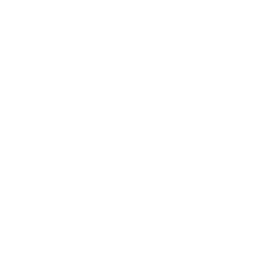
\includegraphics[scale=1]{assets/branding/opa0}
    \vspace{-5.75cm}\\
    {\adjustbox{scale=1.65}{\color{TealDarkCyan}\;III.\;Syndrome Decoding Problem}}
    \vspace{.25cm}
    \begin{minipage}{.78\textwidth}
      \scriptsize\color{Ink}
      \textbf{Big picture.}\;
      Remove the algebraic structure of Hamming and cyclic codes, and the same equation $\mat H\vect e^T=\vect s$ becomes NP-complete.\\[.2cm]
      \textbf{Details to watch.}\;
      random parity-check matrix, weight constraint, NP-completeness, ISD, McEliece, key size.
    \end{minipage}
    {\ }\vspace{2.1cm}\\
    \bigskip
  \end{center}
\end{frame}

%--- The turn: what changes? ---
\begin{frame}{\textbf{III. Syndrome Decoding Problem}}{The Turn: From Structure to Randomness}
\small
\begin{columns}[T,onlytextwidth]
\begin{column}{.50\textwidth}
\textcolor{TealDarkCyan}{\textbf{Structured $\mat H$ (Act II)}}
\begin{itemize}
  \item Columns are all nonzero binary vectors (Hamming).
  \item Generator polynomial of a cyclic ideal (BCH, RS).
  \item Syndrome points to the error address directly.
  \item Decoder runs in $O(1)$ or polynomial time.
\end{itemize}
\end{column}
\begin{column}{.46\textwidth}
\textcolor{TealDarkCyan}{\textbf{Random $\mat H$ (Act III)}}
\begin{itemize}
  \item Each entry of $\mat H$ is an independent uniform bit.
  \item No projective, polynomial, or cyclic structure.
  \item Syndrome gives no algebraic hint about $\vect e$.
  \item Best decoder takes exponential time.
\end{itemize}
\end{column}
\end{columns}
\bigskip
\begin{center}
\begin{tikzpicture}[node distance=.7cm]
  \node[process]          (str)   {structured\\$\mat H$};
  \node[process blue,   right=1.3cm of str]  (sd)    {syndrome\\decoding};
  \node[process amber,  above right=.35cm and 1.3cm of sd] (easy)
    {formula\\$O(1)$};
  \node[process red,    below right=.35cm and 1.3cm of sd] (hard)
    {no formula\\$2^{\Theta(n)}$};
  \node[process,        left=1.3cm of str]   (rand)  {random\\$\mat H$};
  \draw[flow]       (str)  -- (sd);
  \draw[flow]       (rand) -- (sd);
  \draw[flow amber] (sd.north east) -- (easy);
  \draw[flow red]   (sd.south east) -- (hard);
\end{tikzpicture}
\end{center}
\end{frame}

%--- SDP definition ---
\begin{frame}{\textbf{III. Syndrome Decoding Problem}}{The Syndrome Decoding Problem (SDP)}
\defbox[Syndrome Decoding Problem]{
\textbf{Input:}\; $\mat H\in\F_q^{r\times n}$,\; a syndrome $\vect s\in\F_q^r$,\; a weight bound $w\in\N$.\\[4pt]
\textbf{Search:}\; find $\vect e\in\F_q^n$ with
\[
  \mat H\vect e^T = \vect s \quad\text{and}\quad \wt(\vect e)\le w.
\]
\textbf{Decision:}\; does such $\vect e$ exist?
}
\begin{columns}[T,onlytextwidth]
\begin{column}{.50\textwidth}
\textcolor{TealDarkCyan}{\textbf{Parameters}}
\begin{itemize}
  \item $n$: code length
  \item $r=n-k$: redundancy (rows of $\mat H$)
  \item $w$: target error weight
  \item $q=2$: the binary case is most studied
\end{itemize}
\end{column}
\begin{column}{.46\textwidth}
\textcolor{TealDarkCyan}{\textbf{Why hard?}}
\begin{itemize}
  \item $\binom{n}{w}(q-1)^w$ candidates — exponential in $w$
  \item No algebraic shortcut for random $\mat H$
  \item For $n=1024$, $w=50$: $\binom{1024}{50}>10^{80}$
\end{itemize}
\end{column}
\end{columns}
\medskip
\textbf{Comparison.}\; For the $[7,4,3]_2$ Hamming code with $w=1$: only 7 candidates; syndrome names the answer in $O(1)$.
For a random $[1024,512]_2$ code with $w=50$: no formula, only search.
\end{frame}

%--- NP-completeness ---
\begin{frame}[shrink=5]{\textbf{III. Syndrome Decoding Problem}}{NP-Completeness of SDP}
\thmbox[Berlekamp--McEliece--van Tilborg (1978)]{
The decision version of the Syndrome Decoding Problem over $\F_2$ is NP-complete.
}
\begin{columns}[T,onlytextwidth]
\begin{column}{.54\textwidth}
\textbf{Proof sketch (reduction from 3-Dimensional Matching).}
\begin{itemize}
  \item Encode a 3-DM instance as a binary matrix $\mat H$ and syndrome $\vect s$.
  \item A perfect 3-D matching corresponds to a weight-$w$ error with $\mat H\vect e^T=\vect s$.
  \item The reduction is polynomial time.
\end{itemize}
\textbf{Consequence.}\; No polynomial-time algorithm for SDP exists unless $\mathrm{P}=\mathrm{NP}$.

\medskip
\textbf{\color{red}Caution.}\; NP-completeness is a \emph{worst-case} statement.
Cryptographic security requires hardness on \emph{average} for random instances — a separate (conjectured) claim.
\end{column}
\begin{column}{.42\textwidth}
\begin{center}
\begin{tikzpicture}[scale=.80,transform shape,node distance=.60cm]
  \node[process red,minimum width=2.6cm,align=center]     (sat) {3-DM\\(NP-complete)};
  \node[process blue,below=of sat,minimum width=2.6cm,align=center]  (poly){poly-time\\reduction};
  \node[process amber,below=of poly,minimum width=2.6cm,align=center] (sdp) {SDP over $\F_2$\\(NP-complete)};
  \draw[flow red]  (sat) -- (poly);
  \draw[flow blue] (poly) -- (sdp);
  \draw[flow amber,bend left=40]
    (sdp.east) to node[right,tiny label,align=center]{solve\\$\Rightarrow$\\P=NP} (sat.east);
\end{tikzpicture}
\end{center}
\end{column}
\end{columns}
\end{frame}

%--- Visualization: exponential search space ---
\begin{frame}{\textbf{III. Syndrome Decoding Problem}}{The Combinatorial Explosion}
\small
\begin{columns}[T,onlytextwidth]
\begin{column}{.44\textwidth}
For rate $R=1/2$ and error weight $w\approx 0.11n$ (near the Gilbert--Varshamov distance),
the search space is
\[
  \binom{n}{w}\approx 2^{H(w/n)\cdot n}
\]
where $H$ is the binary entropy function.
\medskip

At $n=1000$, $w=110$: $\binom{1000}{110}\approx 10^{100}$ candidates.
\medskip

\textbf{Compare with Hamming.}\; At $n=7$, $w=1$: exactly 7 candidates, resolved by the syndrome in $O(1)$.
\end{column}
\begin{column}{.52\textwidth}
\begin{center}
\begin{tikzpicture}[scale=.70]
  \draw[->,Ink!65] (-.3,0) -- (4.8,0) node[right,tiny label]{$n$};
  \draw[->,Ink!65] (0,-.3) -- (0,3.5) node[above,tiny label]{$\log_2\binom{n}{w}$};
  \draw[TealDarkCyan,thick,domain=.3:4.5,samples=30]
    plot (\x,{0.78*\x}) node[above right,tiny label,TealDarkCyan]{$nH(w/n)$};
  \fill[GoodGreen]  (.10,.08) circle (2.5pt);
  \node[above right,tiny label,GoodGreen]  at (.1,.08) {$n=7$ Hamming};
  \fill[ErrorRed]  (3.5,2.73) circle (2.5pt);
  \node[above right,tiny label,ErrorRed!80]at (3.5,2.73) {$n=1000$};
  \draw[ErrorRed!55,dashed] (0,1.5)--(4.8,1.5)
    node[right,tiny label,ErrorRed!70]{feasible};
  \node[caption text,align=center] at (2.4,-.75)
    {search space grows exponentially in $n$};
\end{tikzpicture}
\end{center}
\end{column}
\end{columns}
\end{frame}

%--- ISD ---
\begin{frame}[shrink=5]{\textbf{III. Syndrome Decoding Problem}}{Information-Set Decoding (ISD)}
\defbox[Prange's Algorithm (1962)]{
Randomly pick $k$ columns $I\subseteq[n]$ so that $\mat H_I$ is invertible (an \emph{information set}).
Assume $\vect e$ is zero on $I$, solve for $\vect e_{[n]\setminus I}=\mat H_{[n]\setminus I}^{-1}\vect s$.
If $\wt(\vect e)\le w$, output $\vect e$.  Otherwise retry.
}
\begin{columns}[T,onlytextwidth]
\begin{column}{.52\textwidth}
\textcolor{TealDarkCyan}{\textbf{Complexity}}
\begin{itemize}
  \item Success probability: $p=\binom{n-w}{k}/\binom{n}{k}$
  \item Cost per trial: $O(n^2)$ (Gaussian elimination)
  \item Total: $\approx O(n^2/p) = 2^{\Theta(n)}$
\end{itemize}
\medskip
\textcolor{TealDarkCyan}{\textbf{Best known ISD variants (binary, rate $1/2$)}}
\begin{itemize}
  \item Stern/Dumer (1989): $\approx 2^{0.054n}$ via birthday trick
  \item BJMM (2012): $\approx 2^{0.049n}$ via representations
  \item Quantum ISD: $\approx 2^{0.027n}$ (Grover, quadratic speedup only)
\end{itemize}
\end{column}
\begin{column}{.44\textwidth}
\begin{center}
\begin{tikzpicture}[node distance=.55cm,scale=.78,transform shape]
  \node[process]              (pick)  {pick info set $I$};
  \node[process blue,below=of pick]  (gauss) {Gauss on $\mat H_I$};
  \node[process amber,below=of gauss](solve) {solve for $\vect e_{[n]\setminus I}$};
  \node[process red,below=of solve]  (check) {$\wt(\vect e)\le w$?};
  \node[process,below=of check,fill=GoodGreen!10,draw=GoodGreen!70] (done) {output $\vect e$};
  \draw[flow]       (pick) -- (gauss);
  \draw[flow blue]  (gauss)-- (solve);
  \draw[flow amber] (solve)-- (check);
  \draw[flow,GoodGreen!80] (check)--node[right,tiny label]{yes}(done);
  \draw[flow red] (check.east)--++(0.5,0)
    |-node[near start,right,tiny label]{no: retry}(pick.east);
\end{tikzpicture}
\end{center}
\end{column}
\end{columns}
\end{frame}

%--- McEliece cryptosystem ---
\begin{frame}[shrink=5]{\textbf{III. Syndrome Decoding Problem}}{McEliece Cryptosystem (1978)}
\defbox[McEliece public-key encryption]{
\textbf{Key generation.}
Choose an $[n,k,d]$ code $\code$ with a $t$-error-correcting decoder (e.g., binary Goppa).
Let $\mat G\in\F_2^{k\times n}$ be its generator.  Choose random invertible $\mat S\in\F_2^{k\times k}$,
random permutation $\mat P\in\F_2^{n\times n}$.  Publish $\hat{\mat G}=\mat S\mat G\mat P$.

\textbf{Encryption.}
$\vect c=\vect m\hat{\mat G}+\vect e$,\; $\vect e$ random with $\wt(\vect e)=t$.

\textbf{Decryption.}
Apply $\mat P^{-1}$, decode $\code$, multiply by $\mat S^{-1}$.
}
\begin{columns}[T,onlytextwidth]
\begin{column}{.50\textwidth}
\textcolor{TealDarkCyan}{\textbf{Security}}
\begin{itemize}
  \item Breaking encryption = decoding $\hat{\mat G}$ without $(\mat S,\mat P)$ = SDP.
  \item Binary Goppa codes: efficient algebraic decoder, resistant to structural attacks.
  \item \textbf{Classic McEliece} is a NIST Round 4 finalist.
\end{itemize}
\end{column}
\begin{column}{.46\textwidth}
\textcolor{TealDarkCyan}{\textbf{Classic McEliece (128-bit)}}
\begin{center}
\renewcommand{\arraystretch}{1.1}
\begin{tabular}{ll}
  $n$ & 3488 \\
  $k$ & 2720 \\
  $t$ & 64 \\
  Public key & $\approx 261\,\text{KB}$ \\
  Ciphertext & $128\,\text{bytes}$ \\
\end{tabular}
\end{center}
\end{column}
\end{columns}
\end{frame}

%--- The cost: large keys ---
\begin{frame}{\textbf{III. Syndrome Decoding Problem}}{The Price of Generality: Large Keys}
\small
\begin{columns}[T,onlytextwidth]
\begin{column}{.52\textwidth}
\textcolor{TealDarkCyan}{\textbf{Why keys are large}}
\begin{itemize}
  \item Security requires $\hat{\mat G}$ to \emph{look random}.
  \item A random $k\times n$ binary matrix has $k(n-k)$ bits.
  \item For rate $R=1/2$: $k(n-k)\approx n^2/4$ bits $= O(n^2)$.
  \item At $n=3488$: $2720\times768 \approx 2.1\times10^6$ bits $\approx 261\,\text{KB}$.
\end{itemize}
\bigskip
\textcolor{TealDarkCyan}{\textbf{The tension}}
\begin{itemize}
  \item SDP hardness demands \emph{no structure}.
  \item No structure means \emph{no compression}.
  \item This is the fundamental trade-off of code-based cryptography.
\end{itemize}
\end{column}
\begin{column}{.44\textwidth}
\begin{center}
\begin{tikzpicture}[scale=.74]
  \draw[->,Ink!60] (0,0)--(0,3.6) node[above,tiny label]{key size};
  \fill[TealDarkCyan!70] (0.4,0) rectangle (1.4,2.8);
  \node[tiny label,align=center] at (.9,-.4) {Classic\\McEliece};
  \node[tiny label,white] at (.9,1.4) {261 KB};
  \fill[BlueCode!70] (2.0,0) rectangle (3.0,0.28);
  \node[tiny label,align=center] at (2.5,-.4) {BIKE};
  \node[tiny label,BlueCode] at (2.5,.52) {1.5 KB};
  \fill[AmberCode!70] (3.4,0) rectangle (4.4,0.52);
  \node[tiny label,align=center] at (3.9,-.4) {HQC};
  \node[tiny label,AmberCode] at (3.9,.76) {3.0 KB};
  \fill[GoodGreen!55] (4.8,0) rectangle (5.8,0.07);
  \node[tiny label,align=center] at (5.3,-.4) {Kyber\\(lattice)};
  \node[tiny label,GoodGreen!80] at (5.3,.3) {1.2 KB};
  \draw[<->,ErrorRed,line width=.8pt] (1.4,2.8)--(3.0,.28)
    node[midway,above right,tiny label,ErrorRed!85!black,rotate=-60]{$\times170$};
  \node[caption text,align=center,text width=4.6cm] at (3.0,-1.05)
    {compact keys require structure — but structure invites attacks};
\end{tikzpicture}
\end{center}
\end{column}
\end{columns}
\medskip
\textbf{The question for Act IV:} Can we add \emph{just enough} structure to compress the key while preserving hardness?
\end{frame}

%--- Complexity landscape ---
\begin{frame}[shrink=5]{\textbf{III. Syndrome Decoding Problem}}{SDP: Complexity Landscape}
\begin{center}
\renewcommand{\arraystretch}{1.24}
\begin{tabular}{p{.26\textwidth}p{.28\textwidth}p{.34\textwidth}}
\toprule
Problem variant & Complexity & Notes \\
\midrule
SDP decision & NP-complete & Berlekamp--McEliece--van Tilborg 1978 \\
SDP search, random $\mat H$, $w\approx\delta_\mathrm{GV}n$ & $2^{0.054n}$ (classical) & Best: Stern, BJMM, May--Ozerov \\
SDP search, quantum & $2^{0.027n}$ & Grover-accelerated ISD; no exponential improvement \\
Minimum distance (find min weight codeword) & NP-hard & Related: $\vect s=\vect 0$ version \\
Structured SDP (cyclic $\mat H$) & Unknown; may be easier & Algebraic attacks possible \\
QC-SDP (quasi-cyclic $\mat H$) & Believed $2^{\Theta(m)}$ & DOOM factor $\sqrt{m}$; Chapter IV \\
\bottomrule
\end{tabular}
\end{center}
\vspace{-.1cm}
\textbf{Summary.}\; SDP is the NP-complete engine at the heart of code-based cryptography.
Its worst-case hardness is proven; its average-case hardness is conjectured and empirically supported by 45 years of failed attacks.
The main weakness: it forces large keys.
Act IV resolves this with quasi-cyclic structure.
\end{frame}
